% Chapter 2 - Social network perspective
\section{Introduction}

Chapter 1 explained how firms engaged in open innovation access knowledge, resources, markets, or technologies via various social networks. The span of a firm’s network of ties to partners (reach) and the resources that the firm can access via its partners (richness) determine the value that it can potentially extract from its inter-organisational networks. Reach and richness bring together structural and relational properties that, together with associated organisational capabilities, help explain the performance implications of social networks \citep{gulati2011networks}. Social network analysis is a tool that allow us to examine network configurations and determine the extent to which these are shaped by individual attributes, contextual factors, and knowledge properties. \medskip

This chapter gives a brief introduction to social network analysis. It kicks off by describing the main characteristics of a social networks. This is followed by an overview of basic network metrics used to identify important individuals in a social network. The chapter then explains what network configurations can reveal about important social network processes. Finally, the chapter introduces exponential random graph models, an advanced social network analysis technique for examining network configurations used in this study. \medskip  

\section{Social networks}

\subsection{Elements of a social network}

A social network is a way to conceptualise a social system in terms of the structure of relationships among social actors. A network can be represented as a mathematical object known as a graph with vertices and edges. The vertices represent actors and the edges the ties between them (Figure \ref{fig:examples}). Actors can be individuals, groups, classes of individuals or other entities. It is the collective action of individual actors that largely determines the global structure of a social network \citep{robins2015doing}. 

\begin{figure}
	\centering
	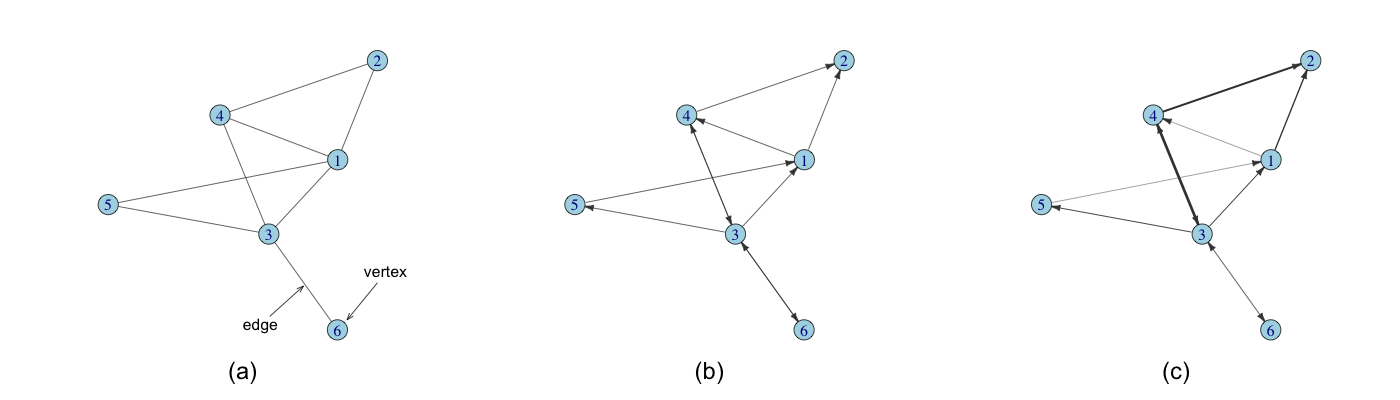
\includegraphics[width=1.0\linewidth]{Images/example_networks.png}
	\caption{Example network with (a) undirected binary ties, (b) directed binary ties, and (c) valued ties (edges are weighted according to some value).}
	\label{fig:examples}
\end{figure}

 Actors may be distinguished by binary, categorical or continuous attributes. For example, consider an individual actor classified as female (binary attribute), who works for a particular organisation (categorical attribute), with a specific number of years work experience (continuous attribute). Ties between actors can be measured as directed or undirected, and as binary or valued. Deciding whether to measure a tie as directed or undirected depends on the nature of the tie. For instance, co-membership is inherently undirected, whereas authority is essentially directed \citep{borgatti2013analyzing}. \medskip
 
 Figure \ref{fig:tie_type} characterises different types of social ties. Ties can be either continuous or discrete in nature \citep{borgatti2013analyzing}. Continuous ties between actors who share something in common (e.g. work at the same location, are affiliated to the same body, participate in the same event, or share a common attribute) are referred to as similarity ties. Relational ties include kinship and other ties, such as friendship, advice, and managerial ties. Relational ties can also be affective (like or dislike another actor) or perceptual (belief about the other actor) in nature. Discrete ties refer to ties defined by specific social interactions (e.g. a transaction of some kind) and flows (e.g. knowledge flows). \medskip

\begin{figure}
	\centering
	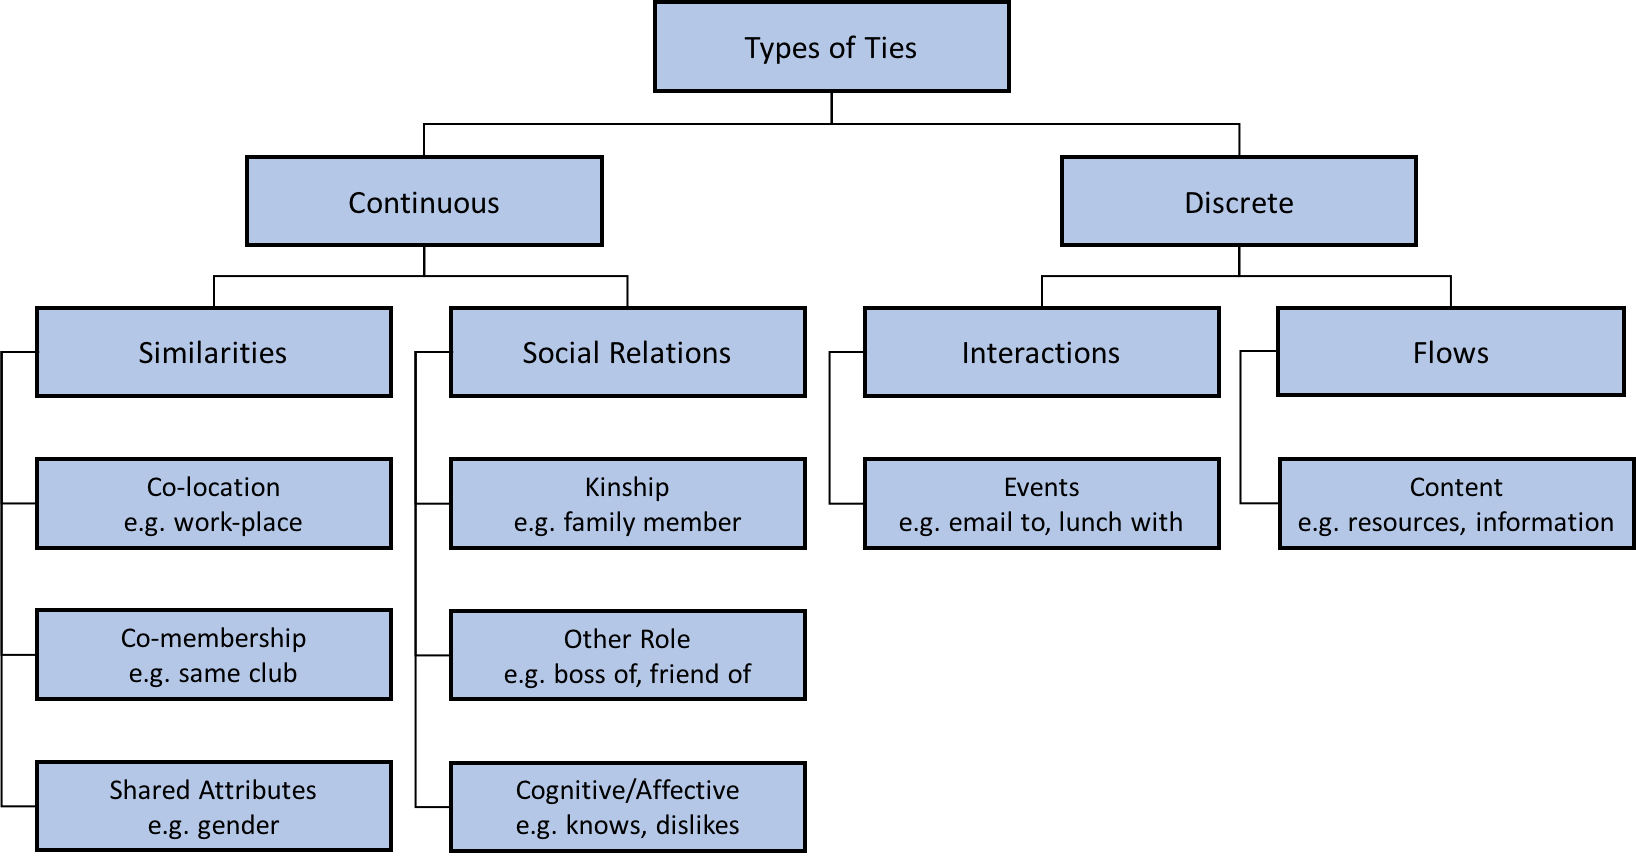
\includegraphics[width=0.9\linewidth]{tie_type}
	\caption{Different types of social ties \citep{borgatti2013analyzing}.}
	\label{fig:tie_type}
\end{figure}

Ties are usually interdependent i.e. the presence of one tie affects the presence of others. Without some form of dependence among ties, it is difficult to reason why certain patterns of ties form \citep{lusher2013exponential}. An example is friendship, which usually develops in the presence of an preexisting similarity tie (e.g. both actors live in the same neighbourhood, attend the same school, or work at the same place) or via a relational event tie (e.g. actors were introduced to each other at a specific event or worked together on a particular project). \medskip

\subsection{Representation of social networks}

A social network can be described as having a given set of $n$ actors, with variables $X_{ij}$ representing how actor $i$ is tied to actor $j$. Edge lists and adjacency matrices are the most commonly used data structures for social networks. With an edge list, an edge between two actors $i$ and $j$ is denoted as $(i,j)$, so that a complete network with $n$ actors can be specified by giving the value $n$ and a list of edges. For example, the edge list for the undirected binary network depicted in Figure \ref{fig:examples} would have $n = 6$ actors and edges $(1,2),(1,3),(1,4),(1,5),(2,4),(3,4),(3,5),(3,6)$. The edge list for the directed binary network would have $n = 6$ actors and edges $(1,2),(1,4),(3,1),(3,4),(3,5),(3,6),(4,2),(4,3),(5,1),(6,3)$. Note that a directed network has twice the number of total possible edges than an undirected network (directed network edges can be bi-directional). \medskip 

Though edge lists are an efficient way to store social network data, they are too cumbersome for computational operations \citep{newman2010networks}. An adjacency matrix is a more efficient way to represent and manipulate social network data \citep{hummon1990computational}. The adjacency matrix of a social network $X$ is an $n \times n$ matrix with elements $X_{ij}$. For a binary network, the adjacency matrix would be expressed as: $$
X_{ij} =
\left \{
  \begin{tabular}{ll}
    1 & if $i$ \rightarrow $j$ \\
    0 & otherwise 
  \end{tabular}
$$ The adjacency matrix for both the undirected and directed binary networks depicted in Figure \ref{fig:examples} would be:$$
X_{ij} =
\left \{
  \begin{tabular}{cccccc}
    0 & 1 & 0 & 1 & 0 & 0 \\
    0 & 0 & 0 & 0 & 0 & 0 \\
    1 & 0 & 0 & 1 & 1 & 1 \\
    0 & 1 & 1 & 0 & 0 & 0 \\
    1 & 0 & 0 & 0 & 0 & 0 \\
    0 & 0 & 1 & 0 & 0 & 0
  \end{tabular}
\right \}
$$ In the case of an undirected network, $X_{ij}$ and $X_{ji}$ are equal. For a directed network, $X_{ij}$ and $X_{ji}$ are different variables, either with the same or different values. With non-binary or valued networks, the presence of a tie is indicated by some value (usually a real number, not equal to 0) that describes a property of the tie e.g. tie-strength, interaction frequency, or some measure of resource exchange. As to the adjacency matrix for a directed binary network, values = 1 in the $i$th row represent ties sent by actor $i$ and the values = 1 in the $j$th column represent ties received by actor $j$. \medskip

Representing ties among actors with matrices can help us measure patterns of social interaction by performing a range of statistical operations based on matrix algebra \citep{anderson1999p}. Examples include counting the number of actual and reciprocated ties ($\sum_{ij}X_{ij}$ and $\sum_{i<j}X_{ji}X_{ij}$, respectively), and calculating the outdegree centrality of the $i$th actor ($X_{i+} = \sum_{j=1}^{n} X_{ij}$). \medskip

\section{Social network analysis}

\subsection{Aim of social analysis}

The primary aim of social network analysis is detecting and interpreting patterns of social ties between actors \citep{de2011exploratory}. The importance of social network analysis rests on three underlying assumptions about patterned relations and their effects. First, structural relations are more important than actor attributes for understanding observed behaviour. For example, an actor may be well-qualified to perform a specific task, but is unable to do the task because the requisite relationships are not in place. Second, social networks shape and are shaped by the perceptions, beliefs, and actions of actors (the \enquote{structure versus agency} debate). Third, structural relations are dynamic i.e. network structures are never static \citep{knoke2008social}. Social network analysis provides a way of looking at a problem but does not predict what we will see. It takes as its starting point the premise that social life is created primarily and most importantly by relations and the patterns they form \citep{scott2011sage}. \medskip

\subsection{Egocentric and sociocentric network analysis}

There are two main types of social network analysis, namely egocentric and sociocentric (also known as whole or complete) network analysis \citep{kilduff2003social}. Egocentric network analysis focuses on the structure of an actor's personal network (the ego's network) and what this means for that actor, whereas sociocentric network analysis considers patterns of social interaction between all the actors in a predefined and bounded population \citep{provan2007interorganizational}. As this study is concerned with tacit knowledge sharing in open innovation partnerships, each with a known number of partner organisations and individual participants, it is sociocentric in nature. \medskip

\subsection{Mixed method social network analysis}

Techniques for analysing social structures have become increasingly mathematical over recent years. However, mathematical techniques do not fully capture the broader context in which social structures emerge \citep{edwards2010esrc}. As mentioned earlier, how people form social relationships is strongly influenced by the perceptions, beliefs, and actions of actors, which may reflect the influence of culture, entrenched social practices, and organisational constraints, amongst other things \citep{dominguez2014mixed}. A mixed method approach enables the exploration of network structure without forsaking the qualitative observations about what is going on within a network \citep{crossley2015cases}. Though social network analysts routinely collect network-related information from individual informants, much of this information is prone to bias or misrepresentation \citep{williams2017mixed}. Mixed method social network analysis combines quantitative and qualitative approaches in more rigorous ways to better understand the practices and conditions that produce certain network outcomes \citep{dominguez2014mixed}. \medskip

\section{On the nature of knowledge}

Before delving into how motivation, trust, and power influence knowledge sharing behaviour, it is important to clarify what knowledge is and understand what knowledge management is about. \citet{davenport1998working} define knowledge as \enquote{a fluid mix of framed experience, values, contextual information, and expert insight that provides a framework for evaluating and incorporating new experiences and information}. \citet{leonard1998role} refers to knowledge as \enquote{information that is relevant, actionable, and at least partially based on experience}. Both \citet{davenport1998working} and \citet{leonard1998role} emphasise the importance of tacit knowledge. \medskip

Knowledge management is primarily about translating individual or group learning into organisational capability \citep{mcdermott1999information,hansen2005share,lam2010knowledge,girard2015defining}. It revolves around managing people or information \citep{alvesson2001odd}. Unless a person or a group decides to share their knowledge, it remains a hidden and untapped resource \citep{davenport1998working}. Knowledge sharing can be understood as the behaviour by which an individual or group voluntarily provides others with access to their unique knowledge and experiences \citep{cabrera2002knowledge,hansen2005share}. More explicitly, knowledge sharing refers to \enquote{the provision of task information and know-how to help others and to collaborate with others to solve problems, develop new ideas, or implement policies or procedures} \citep{wang2010knowledge}.
Individuals or groups who share their knowledge contribute to the competitive advantage of organisations \citep{papadopoulos2013exploring}. \medskip


\subsection{Network metrics}

\subsubsection{Density}

Density measures the overall level of connectivity in a social network. It is simply the proportion of actual (observed) ties to total number of possible ties:  $$\rho = \frac{\sum_{ij}^{n}X_{ij}}{n(n-1)}(i \neq j)$$ where $\rho$ is network density, $\sum_{ij}^{n}X_{ij}$ is the number of observed ties, and $n(n-1)$ is the total number of possible ties. Density ranges from 0 (nobody is connected) to 1 (everybody is connected to one another). The denser the network, the higher the level of social cohesion in the network \citep{newman2010networks}. Information in dense networks can flow more easily than information in sparse networks \citep{borgatti2013analyzing}. \medskip

\subsubsection{Centrality}

Centrality is a property of an actor's position in a network. One can think about centrality in terms of the contribution an actor makes to the structure of the network \citep{borgatti2013analyzing}. There are many ways to measure centrality, each focused on a different aspect of centrality \citep{freeman1979centrality}. The simplest measure is degree centrality, which measures an actor's connectivity by counting the number of ties they have with other actors. For an undirected network with \(n\) actors, degree centrality is calculated as follows: $$ d_i=\sum_{j=1}^{n}x_{ij}(i \neq j) $$ where $d_i$ is the degree centrality for actor $i$ and $\sum_{j=1}^{n}(x_{ij})$ counts the number of direct ties that $i$ has to $n-1$ other $j$ actors. Actors with higher degree values are more connected than those with lower values. High degree centrality represents an opportunity to influence and be influenced directly \citep{borgatti2013analyzing}. Directed networks have out-degree and in-degree centrality (number of ties directed away from and towards an actor, respectively). In-degree centrality is an indicator of an actor's popularity, whereas out-degree centrality is an indicator of an actor's social activity \citep{robins2015doing}. Closeness centrality measures how near an actor is to other actors in the social network and is calculated as the sum of the length of the shortest paths between the actor and all other actors in the network: $$c_i=\frac{1}{\sum_{j}^{n}d(i,j)}(i \neq j)$$ where $c_i$ is the closeness centrality for actor $i$ and $d(i,j)$ is the distance between actors $i$ and $j$. Closeness indicates how quickly an actor can interact with others or diffuse information through the network e.g. by communicating either directly or through very few intermediaries \citep{bavelas1950communication,freeman1979centrality,knoke2008social}. Another centrality measure is betweenness, which measures the extent to which an actor lies on paths between other actors: $$ b_i=\sum_{i < k}\frac{g_{jik}}{g_{jk}} $$ where $b_i$ is the betweenness centrality for actor $i$, $g_{jik}$ is the number of shortest paths connecting $j$ and $k$ through $i$, and $g_{jk}$ is the total number of shortest paths connecting $j$ and $k$ \citep{freeman1979centrality}. Betweenness is an important measure of an actor's control over (or ability to broker) information exchange or resource flows within a network \citep{knoke2008social,everett2016bridging}. An actor with high betweenness often bridges otherwise disconnected parts of the network. Their removal from the network can severely disrupt network communication \citep{borgatti2013analyzing}. Eigenvector centrality is a measure of an actor's influence in the network \citep{bonacich1987power}. For a given network $X$, the eigenvector centrality $e_{i}$ of node $i$ is given by: $$e_i = \frac{1}{\lambda} \sum_j X_{ij}e_j$$ where $\lambda \neq 0$ is a constant. In matrix form we have: $$\lambda e = Xe$$ An actor with high eigenvector centrality is connected to other well-connected actors in the network and thus has greater influence. Eigenvector centrality tends to identify centres of large cliques \citep{borgatti2013analyzing}. \medskip

\subsubsection{Constraint}

\citet{burt1992structural} measures an actor's brokerage opportunities in terms of \enquote{network constraint}, a summary index that quantifies the extent to which an actor's access to network resources is constrained. Network constraint is calculated as follows: $$ C_i = \sum_j c_{ij} (i \neq j) $$ where $C_i$ is the network constraint on actor $i$ and $c_{ij}$ is a measure of $i$'s dependence on $j$: $$ c_{ij} = (p_{ij} + \sum_qp_{iq}p_{qj})^2 (i \neq q \ne j) $$ and $p_{ij}$ is the proportion of $i$'s time and energy spent on $j$: $$ p_{ij} = \frac{z_{ij}}{\sum_qz_{ig}} $$ where variable $z_{ij}$ measures the strength of the tie between $i$ and $j$. Network constraint is high if the actor has few but strong ties \citep{burt2010neighbor}. An actor with low network constraint has greater access to distant network resources through a higher number of weak ties \citep{granovetter1973strength}. \medskip

\subsection{Social network processes}

Sociologists increasingly agree that social life is shaped by a limited number of social mechanisms or processes \citep{crossley2015cases}. Unpacking a social system into constituent elements for analysis is challenging, given the interdependence of social ties \citep{robins2015doing}. Take friendship for example. As mentioned earlier, friendship ties often form in the presence some existing similarity tie. At the same, friendship usually has to be reciprocated for it to be sustained \citep{hartup1996company,almaatouq2016role}. Friendship also tends to lead to the formation of cliques i.e. \enquote{a friend of a friend is a friend of mine} \citep{lusher2013exponential}. The interdependence of ties can lead to complex feedback mechanisms that make interpretation of social network processes difficult \citep{robins2015doing}. Any attempt to make sense of social network processes must have a solid theoretical basis i.e. be based on a set of theoretical assumptions to best describe and explain social phenomena of interest \citep{borgatti2013analyzing}. This usually involves developing propositions or testing hypotheses about specific social network processes based on existing psychological or social theories \citep{scott2017social}. \medskip

Overviews of some key social network processes and their theoretical basis are presented below. The aim is not to provide an exhaustive list of social network processes. Rather, it is to introduce key social network processes that are particularly relevant to this study, namely reciprocity, network closure, tie-strength, preferential attachment, and brokerage. For a more complete exposition of social network processes, the reader is referred to  \citet{burt2005brokerage}, \citet{knoke2008social}, \citet{de2011exploratory}, \citet{kadushin2012understanding}, and \citet{scott2017social}. \medskip

\subsubsection{Reciprocity}

Reciprocity (\(X_{ij}X_{ji}\)) is a common feature of social networks. Both social exchange and game theory suggest dyadic relationships have a tendency to be reciprocal \citep{emerson1976social,axelrod1984evolution}. Reciprocity reflects a human tendency to return helpful (or harmful) acts in kind e.g. \enquote{you scratch my back because I have scratched yours} \citep{nowak2005evolution}. Reciprocity contributes to more balanced and stable social relations, which in turn helps build trust and strengthen ties between actors \citep{blau1964exchange}. \medskip

\subsubsection{Preferential attachment}

New actors joining a network tend to connect with other actors who are highly visible due to their popularity \citep{desollaprice976general}. This attachment bias is referred to as \enquote{preferential attachment} \citep{barabasi1999emergence}, where the probability of \(j\) forming a tie with \(i\) is dependent on the degree \(k_{i}\) (for undirected networks \(P(k_{i})=\frac{k_{i}}{\sum_{j}k_{j}}\)). Such bias means that popular actors will increase their connectivity at a higher rate than less popular actors, the so-called \enquote{rich-get-richer} phenomenon \citep{desollaprice1976general,adamic2000power,easley2010power}.  Preferential attachment leads to positively skewed degree distributions, with a small number of actors with very high degree centrality and many actors with lower degree centrality. This has implications for the concentration of power in social networks \citep{emerson1962power}. \medskip 

\subsubsection{Network closure}

Network closure reflects a human tendency to operate in small groups (also referred to as \enquote{cliques}). Balance theory argues unbalanced relations are stressful for humans. To reduce stress, humans strive for structural balance in social relations. This usually leads to the formation of triangular social structures through a process known as transitive closure. Triangles can be thought of as archetypal small groups \citep{robins2015doing}. In the case of directed networks, transitive closure can be either cyclic or hierarchical in nature \citep{davis1967structure}. With cyclic closure, each actor in the triad has one incoming and one outgoing tie (\(X_{ij}X_{jk}X_{ki}\)). Actors are structurally equivalent and engaged in \enquote{generalised exchange}. This is not the case with hierarchical closure, where one actor in the triad has two incoming ties (\(X_{ij}X_{jk}X_{ik}\)), evidence of a local hierarchy. Empirical studies indicate that cyclic closure is less prevalent in social networks, pointing to the pervasiveness of hierarchies in local group structures \citep{davis1967structure}. \medskip

\subsubsection{Homophily}

Homophily is the principle that contact between similar people occurs at a higher rate than among dissimilar people \citep{mcpherson2001birds}. It is not that much different to preferential attachment. If preferential attachment considers popularity to be attractive, similarity might be another dimension of attractiveness \citep{wang2014homophily}. In essence, homophily implies that the distance in social characteristics translates into network distance (the number of steps or links between two actors) i.e. the greater the similarity between actors, the shorter the network distance between them. This has implications for the information people receive, the attitudes they form, and the interactions they experience \citep{mcpherson2001birds}. Apart from limiting access to more diverse information, homophily also promotes network closure \citep{kossinets2009origins}. Though homophily may indicate a preference to connect with similar others, the underlying motives for this are not well understood. \citet{kets2016belief} argue homophily is ultimately driven by an innate need to reduce uncertainty. Homophily emerges because players find it easier to predict the instinctive reactions of members of their own group. So while homophily may limit social reach, it does contribute to more balanced and stable social relationships \citep{scott2011sage,baccara2013homophily}. \medskip

\subsubsection{Strong and weak ties}

Actors who know each other well are said to have \enquote{strong} ties with one another. Multiplex relations between two actors are also considered to be stronger because their redundancy can make them endure the break-up of a specific type of relation \citep{dickison2016multilayer}. Casual acquaintances, on the other hand, can be regarded as \enquote{weak} ties. Strong ties usually lead to transitive closure, resulting in people becoming more inward looking and less receptive to external knowledge. Because acquaintances usually mix in different social circles, weak ties are more likely to provide actors greater access to new knowledge and opportunities \citep{granovetter1973strength}. Although weak ties enhance connectivity across the network, strong ties tend to be more effective than weak ties in facilitating learning and getting things done \citep{ahuja2000collaboration,burt2004structural,rost2011strength,phelps2012knowledge}. \medskip

\subsubsection{Brokerage}

Brokerage may be defined as the \enquote{behaviour by which an actor influences, manages, or facilitates interactions between other actors} \citep{obstfeld2014brokerage}. Actors that bridge otherwise disconnected parts of the network are said to occupy \enquote{structural holes} in the network \citep{burt1992structural}. They have high betweenness centrality or low network constraint and are able to control or broker information exchange or resource flows through their network of weak ties. Actors occupying structural holes are well-placed to extract better bargains in exchanges, exert greater influence, and be a focus of attention from those in less favoured positions \citep{burt1992structural,hanneman2005introduction,simpson2011network}. They can exploit their favoured position either to gain some form of personal advantage (known as \textit{tertius gaudens} brokerage), or to facilitate new social relations (referred to as \textit{tertius inungens} brokerage) \citep{obstfeld2005social,obstfeld2014brokerage,quintane2016brokers}. \medskip 

\section{Exponential random graph models}

\subsection{Overview}

Exponential random graph models (ERGMs) are a class of statistical model for social networks. The model represents a network as an accumulation of local \enquote{network configurations} (also referred to as \enquote{subgraphs}, \enquote{motifs}, or \enquote{microstructures}) that build the global structure of the network \citep{robins2013tutorial}. Network configurations are local patterns of social network ties assumed to represent underlying social processes or mechanisms \citep{lusher2013exponential}. \medskip

ERGMs are based on the premise that network ties depend on one another i.e. the presence of one tie may affect the presence of others. ERGMs are theory-driven in that their use requires the researcher to consider the complex, intersecting, and often competing theoretical reasons why particular social ties in the observed network exist \citep{lusher2013exponential}. For instance, does a given network structure occur due to processes of homophily, reciprocity, transitivity, or through a combination of these? By including such parameters together in one model, a researcher can test certain hypotheses or propositions about tie formation relating to theory \citep{robins2007recent}. Alternative methods used to assess the effect of actor attributes on network structures, such as linear regression, are unable to make such distinctions, and are thus more limited regarding the conclusions such methods can draw. \medskip

ERGMs can distinguish between ties formed due to actor attributes or whether an actor’s centrality is the result of being embedded within other purely structural network structures \citep{lusher2013exponential}. Purely structural effects reflect self-organising or endogenous processes where ties form due to the presence or absence of other ties e.g. reciprocity and transitive closure. Actor-relation effects refer to ties that form due to actor attributes. Homophily is an example of an actor-relation effect.  Dyadic covariate effects refer to ties in one network being affected by ties in another network. A good example is geographic distance between actors, which may affect the formation of relationships between them. Another example is advice seeking, which is more likely to occur in the presence of an existing friendship tie. \medskip

\subsection{Statistical representation}

Statistically, an ERGM represents a probability distribution of graphs for a given set, where the probability of observing a graph is dependent on the presence of the various network configurations expressed by the model. For a binary network, the probability of observing specific network configurations for a given set of actors \(n\) can be expressed as follows: $$ P(X = x) = \frac{\exp \left \{ \theta'z(x)  \right \}}{\kappa (\theta )} $$ where $P(x)$ indicates the probability of a given network, $\theta$ indicates a vector of model parameters, $z(x)$ is a vector of network statistics, and $\kappa$ is a normalising function to ensure a proper probability distribution across a set of random networks \citep{shumate2010exponential}. Network statistics $z(x)$ are counts of the estimated number of configurations in the network, or some function of those counts. The probability of the network depends on how many of those configurations are present and the parameters indicate the importance of each configuration \citep{lusher2013exponential}. Large positive parameters suggest that more configurations of that type are observed in the network than expected by chance alone \citep{robins2009closure}. One limitation of ERGMs is that the algorithms used to estimate model parameters often fail to converge. For this reason ERGMs tend to be parsimonious, including only the most important configurations needed to answer specific questions \citep{mcallister2017balancing}. \medskip

\begin{figure}
	\centering
	\small
	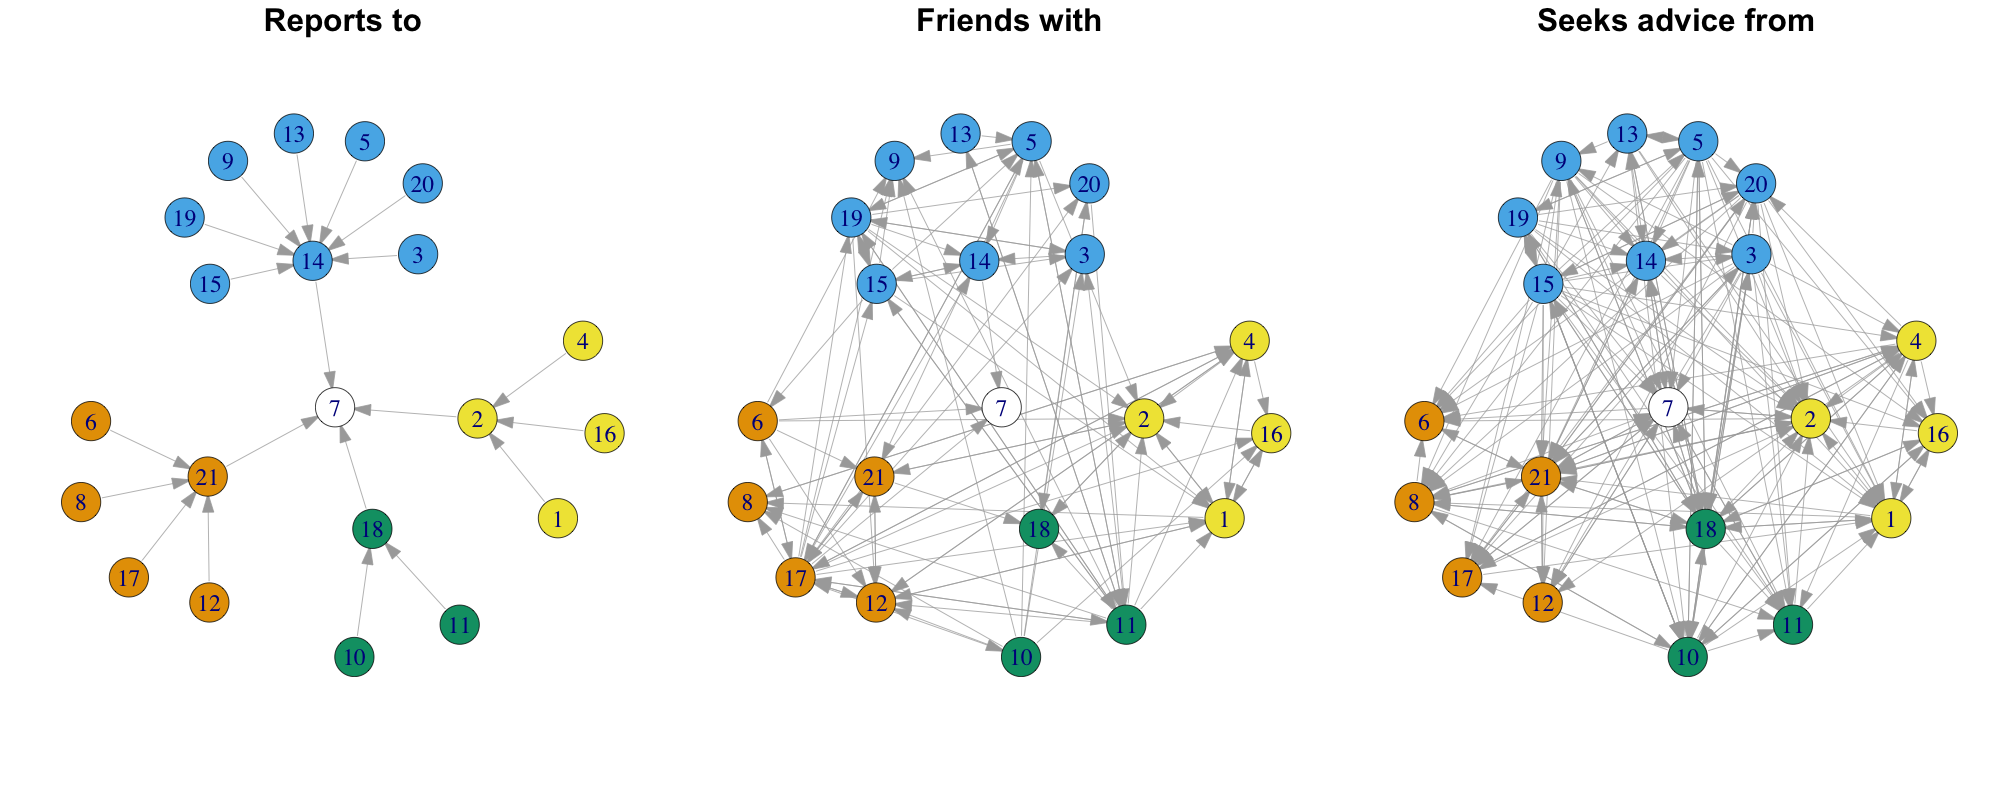
\includegraphics[width=1.0\linewidth]{Images/krackhardt.png}
	\caption{Reporting, friendship, and advice-seeking networks in a high-technology firm. Node colours indicate membership of different organisational units. Data from \citet{krackhardt1990assessing}.}
	\label{fig:krackhardt}
\end{figure}

\subsection{Example ERGM analysis}

The best way to demonstrate how an ERGM works in practice is through a simple real-world example. Figure \ref{fig:krackhardt} shows reporting, friendship, and advice-seeking relations among 21 senior managers at a high-technology firm in the USA. The network data is from a well-known study conducted by \citet{krackhardt1990assessing}. Though the network diagrams show how the managers are connected with each other, which ties are reciprocated, and who is central in each network, they reveal little about the social processes that shape advice-seeking relations e.g. does age or experience matter in advice-seeking? In our simple example, we use an ERGM to test three simple propositions that might explain how advice-seeking relations develop: 

\begin{itemize}[label={},leftmargin=0pt]
    \item \textit{Proposition 1: Because people tend to seek advice from others they trust, managers are more likely to seek advice from those they regard as friends.}
    \item \textit{Proposition 2: Assuming highly-competent people get promoted to more senior management positions, they are more likely be approached by their subordinates for advice.}
    \item \textit{Proposition 3: Because relevant expertise or know-how takes time to accumulate, managers are more likely to seek advice from others who have been with the firm longer.}
\end{itemize}

We explicitly model the following effects in the advice-seeking network: co-entrainment of friendship and reporting relations (dyadic covariate effect) and a receiver effect for tenure (actor-relation effect). Control variables include arc, reciprocity, popularity spread, transitive (path) closure, and cyclic closure (purely structural effects), and age difference (actor-relation effect). Not only does our ERGM converge successfully, the goodness of fit is excellent, with 95\% of the non-explicitly modelled parameters having a t-ratio of less than 2. The goodness of fit tells us that we can explain the global structure of the advice-seeking network using our small number of explicitly modelled parameters. Modelling results are presented in Table \ref{ERGM_example}.

\begin{landscape}
    \begin{table}[]
    \small
    \centering
    \caption{Example ERGM analysis: Advice-seeking in a high technology firm.}
    \label{ERGM_example}
        \begin{tabular}{lcp{10cm}rl}
            \toprule
            Parameter & Configuration & Explanation & \multicolumn{2}{r}{Estimate (SE)} \\ \midrule
            \multicolumn{5}{l}{\textbf{Purely structural effects}} \\
            Arc & \begin{minipage}{.2\textwidth} \centering 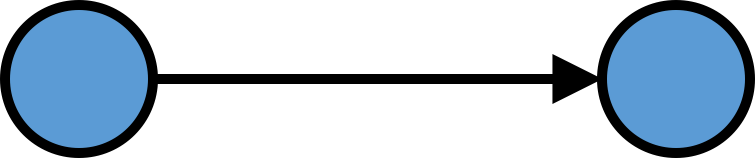
\includegraphics[width=0.45\linewidth]{Images/Arc} \end{minipage}  & Baseline propensity for a tie to form in the absence of other effects. & 1.42 & (2.87) \\
            Reciprocity & \begin{minipage}{.2\textwidth} \centering 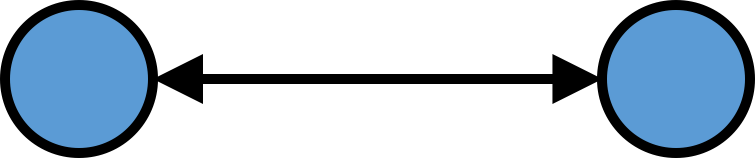
\includegraphics[width=0.45\linewidth]{Images/Reciprocity} \end{minipage}  & Propensity for a tie from one actor to a second when there is already a tie from the second to the first. & 0.71 & (0.33)* \\
            Popularity spread & \begin{minipage}{.2\textwidth} \centering 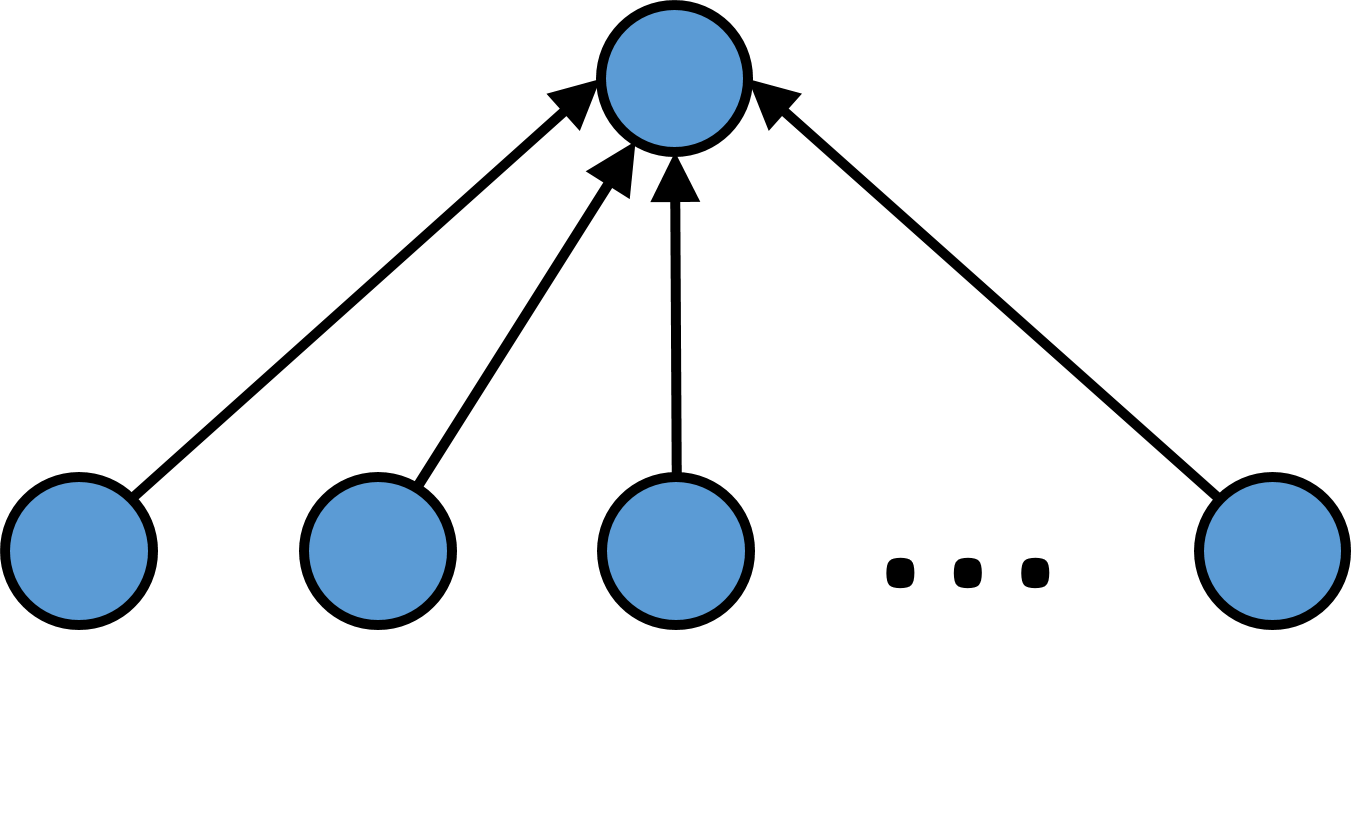
\includegraphics[width=0.8\linewidth]{Images/AinS} \end{minipage}  & Propensity for dispersion in the in-degree distribution, indicating there are few highly poplar actors. & 1.77 & (1.48) \\
            Hierarchical closure & \begin{minipage}{.2\textwidth} \centering 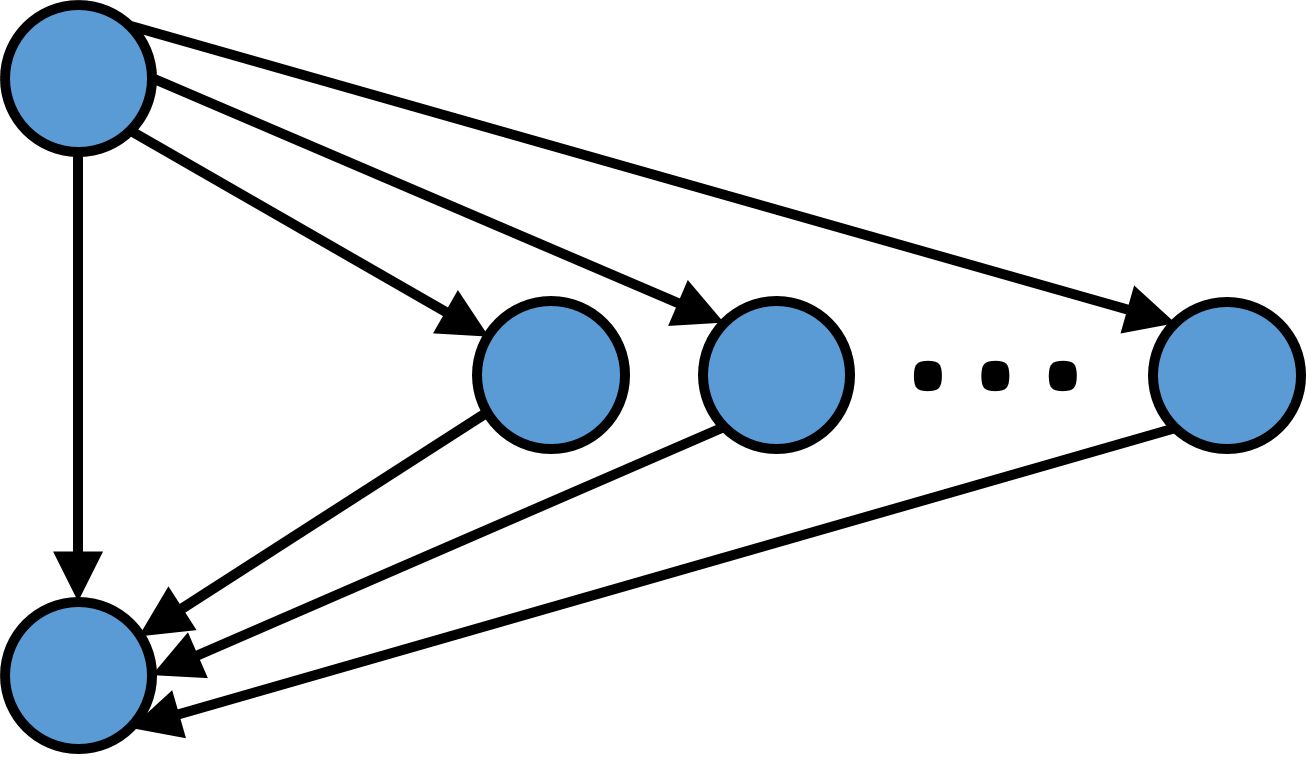
\includegraphics[width=0.8\linewidth]{Images/AT-T} \end{minipage} & Propensity for ties to form as part of a hierarchical triad or a multiple hierarchical configuration. & 1.00 & (0.25)* \\
            Cyclic closure & \begin{minipage}{.2\textwidth} \centering 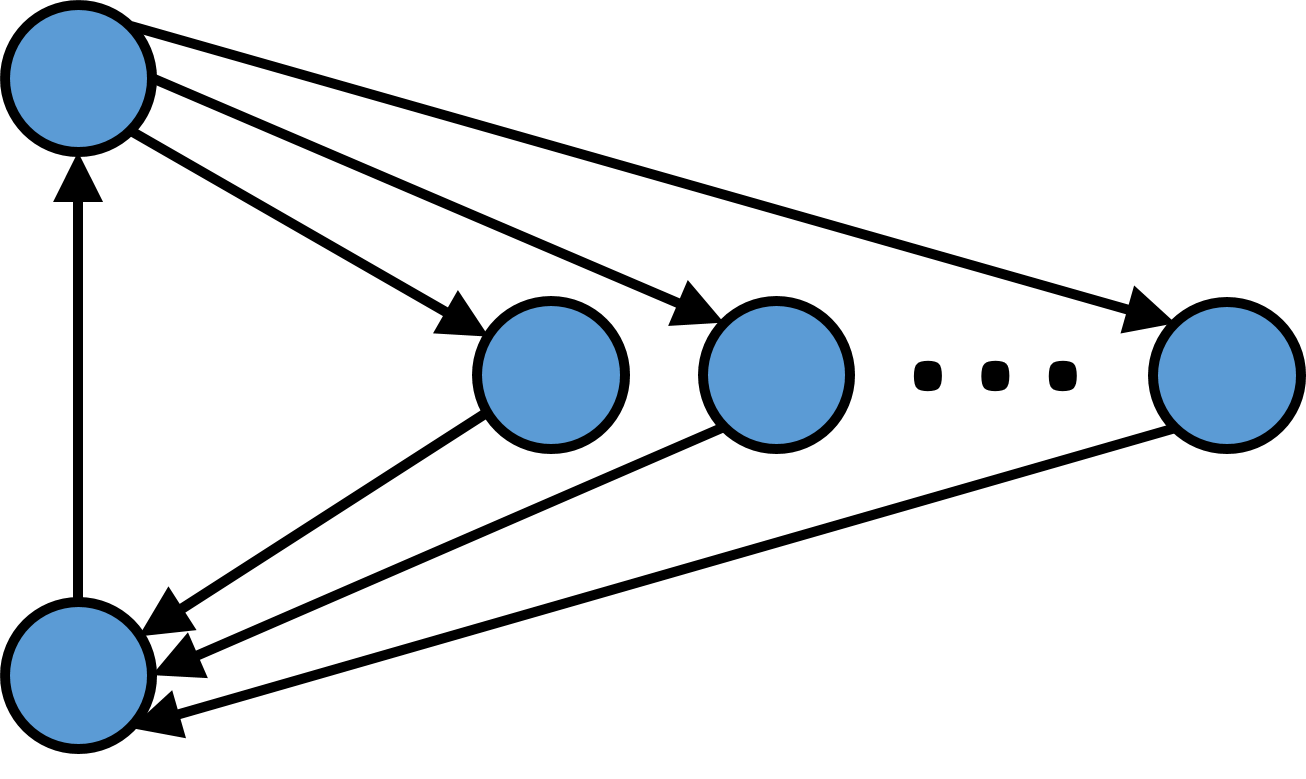
\includegraphics[width=0.8\linewidth]{Images/AT-C} \end{minipage} & Propensity for ties to form as part of a cyclic triad or a multiple cyclic configuration. & -0.50 & (0.06)* \\ \\
            \multicolumn{5}{l}{\textbf{Actor-relation effects}} \\
            Attribute difference (Age) & \begin{minipage}{.2\textwidth} \centering 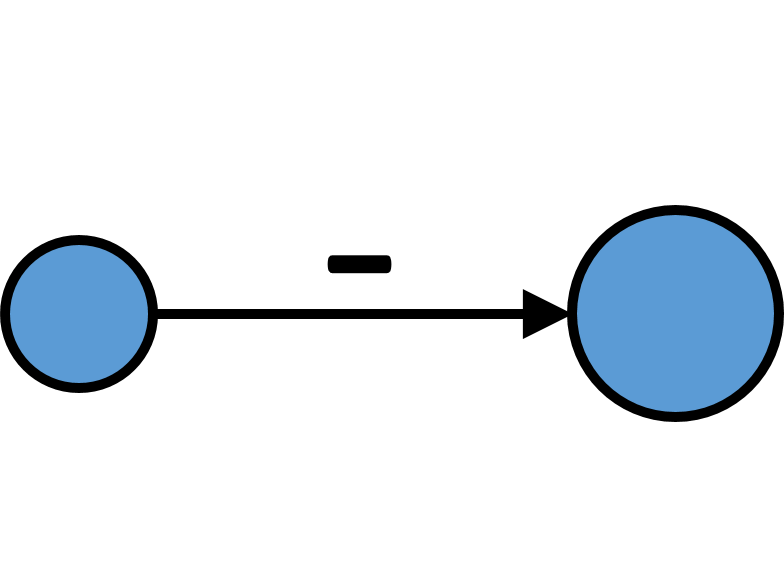
\includegraphics[width=0.45\linewidth]{Images/Difference} \end{minipage} & Propensity for a tie to form between actors of a similar age. & -0.03 & (0.01)* \\
            Attribute receiver (Tenure) & \begin{minipage}{.2\textwidth} \centering 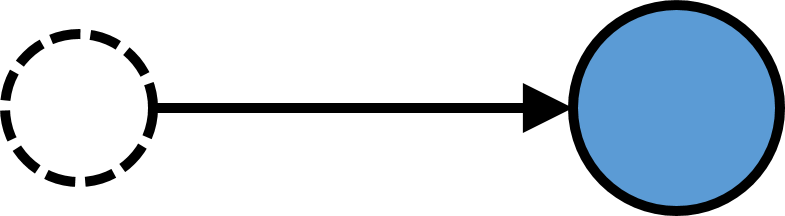
\includegraphics[width=0.45\linewidth]{Images/Receiver} \end{minipage} & Propensity for a tie to be directed toward an actor with longer tenure. & 0.05 & (0.02)* \\ \\
            \multicolumn{5}{l}{\textbf{Dyadic covariate effects}} \\
            Co-entrainment (Reports to) & \begin{minipage}{.2\textwidth} \centering \vspace{0.5cm}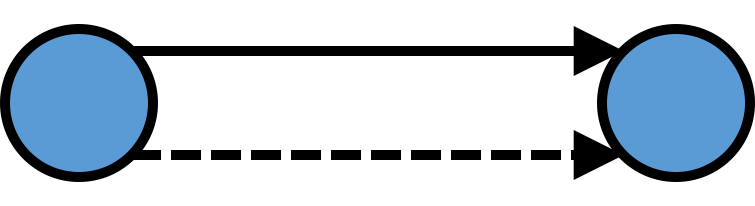
\includegraphics[width=0.45\linewidth]{Images/DyadicCovariate} \end{minipage} & Propensity for a tie of one type to form from one actor to another if a reporting tie is already present. & 0.55 & (0.51) \\
            Co-entrainment (Friends with) &  & Propensity for a tie of one type to form from one actor to another if a friendship tie is already present. & 0.55 & (0.22)* \\ \bottomrule
        \end{tabular}
    \end{table}
\end{landscape}

The significant and positive effect for reciprocity indicates advice-seeking is mutual i.e. advice-seeking tends to be reciprocated, potentially a sign of mutual trust \citep{blau1964exchange,axelrod1984evolution}. There is also a significant and positive effect for transitive closure and significant and a negative effect for cyclic closure in the advice-seeking network. Not only does this indicate advice-seeking is triadic in nature, it also suggests advice-seeking is targeted and not generalised i.e. advice is mostly sought from a specific person in a group (a sign of local deference). The significant and negative age difference effect indicates managers are inclined to seek advice from others of a similar age (an age-homophily effect). Moreover, there is a significant and positive receiver effect for tenure, which validates the proposition that managers are more likely to seek advice from others who have been with the firm for longer. The significant and positive co-entrainment effect for friendship supports the proposition that managers are more likely to seek advice from others they regard as friends (another sign that advice-seeking involves trust). Not supported is the proposition that managers are likely to seek advice from their immediate managers i.e. there is no significant dyadic co-entrainment effect for the reporting network. \medskip

The ERGM analysis shows that the managers at the high-technology firm tend to seek advice from colleagues they regard as friends, who are of a similar age, and who have been with the firm for longer. They can expect to be asked for advice in return. Reciprocity, transitive closure, and friendship suggest advice-seeking is trust-based. Hopefully, this simple example demonstrates the explanatory power of ERGMs in social network analysis. \medskip

\section{Conclusion}

Social network analysis allows one to use centrality measures to identify important actors in open innovation networks and to assess knowledge sharing behaviour in such networks by examining specific network configurations. The interdependence of social relations can lead to complex feedback mechanisms that make interpretation of social network processes difficult. Exponential random graph models (ERGMs) are a class of statistical model for social networks that breaks a network down into its constituent network configurations. Network configurations are assumed to represent underlying social processes or mechanisms. An ERGM allows a researcher to test hypotheses or propositions about network tie formation that relate to social theory. The following chapter (Chapter 3) reviews key social theories pertinent to this study, theories that can help explain knowledge sharing behaviour in open innovation partnerships. 